% ---------------- RELAZIONE PROGETTO DI PROGRAMMAZIONE AD OGGETTI (OOP) --------
\documentclass[a4paper,12pt]{report}

% ----------------------------- PREAMBLE --------------------------------------- 

\usepackage{lmodern}
\usepackage{alltt, fancyvrb, url}
\usepackage{float}
\usepackage{geometry}
\usepackage{graphicx}
\usepackage[utf8]{inputenc}
\usepackage{hyperref}
\usepackage{amsmath,amssymb,amsthm}
\usepackage{layout}
\usepackage[italian]{babel}
\usepackage[italian]{cleveref}
\usepackage{comment}
\usepackage{microtype}
\usepackage{fancyhdr}
\usepackage[scaled=.92]{helvet}
\usepackage[T1]{fontenc}
\usepackage{lscape}
\usepackage{listings}
\usepackage{color}
\definecolor{dkgreen}{rgb}{0,0.6,0}
\definecolor{gray}{rgb}{0.5,0.5,0.5}
\definecolor{mauve}{rgb}{0.58,0,0.82}

\lstset{frame=tb,
	language=Java,
	aboveskip=3mm,
	belowskip=3mm,
	showstringspaces=false,
	columns=flexible,
	basicstyle={\small\ttfamily},
	numbers=none,
	numberstyle=\tiny\color{gray},
	keywordstyle=\color{blue},
	commentstyle=\color{dkgreen},
	stringstyle=\color{mauve},
	breaklines=true,
	breakatwhitespace=true,
	tabsize=3
}


% hyperref settings
\hypersetup{
	colorlinks=true,
	linkcolor=black, %blue
	filecolor=magenta,      
	urlcolor=cyan,
	pdftitle={Sharelatex Example},
	bookmarks=true,
	pdfpagemode=FullScreen,
}

\geometry{
	a4paper,
	total={170mm,257mm},
	left=20mm,
	top=20mm,
}

% ----------------------------- PREAMBLE END -----------------------------------

\makeindex

\title{\textbf{Crittografia}}
\author{Alessandro Pioggia, Luca Rengo, Federico Brunelli, Leon Baiocchi}


\begin{document}
	\makeatletter
	\begin{titlepage}
		\begin{center}
			{\Huge  \@title }\\[3ex] 
			{\large  \@author}\\[3ex] 
			{\large \@date}
		\end{center}
	\end{titlepage}
	\makeatother
	\thispagestyle{empty}
	\newpage
	
	%\maketitle
	
	\tableofcontents
	
	% \input: import the commands from filename.tex to target file.
	
	% \include: does a \clearpage and does an \input.
	
	\newpage
	
	\chapter{Introduzione}

Impariamo due nozioni di crittografia in caso servano per le comunicazioni della terza guerra mondiale.
	
	\chapter{One-time pad}

\begin{lstlisting}
	//Hello.java
	import javax.swing.JApplet;
	import java.awt.Graphics;
	
	public class Hello extends JApplet {
		public void paintComponent(Graphics g) {
			g.drawString("Hello, world!", 65, 95);
		}    
	}
\end{lstlisting}
	
	\chapter{Il caso}

La randomness è la regina della crittografia, è vista come una risorsa, costa e richiede energie per produrla : più la randomness è randomica, più i protocolli sono sicuri. 

\section{Bit casuale}

Un bit casuale è un qualcosa che può assumere valore 0 o 1 con probabilità $\dfrac{1}{2}$, questa definizione ci porta però a scontrarci con questa situazione:
\begin{itemize}
	\item sequenza 1 : 11111111
	\item sequenza 2 : 10100100
\end{itemize}
Notiamo che la prima sequenza non è casuale mentre la seconda sì (per la legge dei grandi numeri la prima è molto improbabile che sia casuale, specie se estesa ad un numero di cifre alto).
Ma secondo la prima definizione che abbiamo dato considera che $P(11111111) = P(10100100) = \dfrac{1}{2^{10}}$, il che non è in linea con il nostro ragionamento.

\section{Casualità in crittografia}

In crittografia casuale = "non facilmente prevedibile", un ipotetico avversario (o intruso) non deve essere in grado di prevedere ciò che noi generiamo a caso.

\section{Casualità secondo Laplace}
Laplace osserva che se tu lanci 100 volte una moneta, le combinazioni di risultati (T o M), formano sequenze regolari, facili da comprendere oppure sequenze irregolari che sono incomparabilmente più numerose (ci sono più combinazioni irregolari rispetto a quelle regolari).

\section{Casualità secondo Kolmogorov}
Kolmogorov dice che una sequenza binaria h è casuale se non ammette alcun algoritmo di generazione A la cui rappresentazione binaria sia più corta di h.
Se noi prendessimo le cifre dopo la virgola di $\pi$ notiamo che queste sono abbastanza irregolari. Noi possiamo però creare un programma che, a seconda della complessità, mi può restituire le cifre di $\pi$ sempre più grandi (il programma però ha una lunghezza finita!). Secondo Kolmogorov quindi, la generazione di $\pi$ non è casuale, le cifre dopo la virgola è possibile determinarle in maniera assoluta da un programma di lunghezza costante. Kolmogorov introduce il concetto di complessità computazionale, se ho un algoritmo definito che genera una stringa, in maniera deterministica, non si può parlare di casualità.

\subsection{Riflessioni}

Supponiamo di avere una procedura Random(n) che produce una sequenza di n bit. Quando n cresce le sequenze prodotte da Random non saranno casuali avendo una lunghezza maggiore della rappresentazione binaria della procedura Random. 

\paragraph{Quindi} secondo Kolmogorov non esistono generatori di
numeri casuali!!!

\section{Pseudo-casualità}

Noi abbiamo bisogno di casualità, è la nostra risorsa, quindi sarà necessario considerare il concetto di \textbf{pseudo-casuale} (quasi casuale). I generatori pseudo-casuali sono algoritmi che producono sequenze di bit che supereranno i test di casualità.
I test di casualità sono proprietà che le stringhe prodotte dai generatori devono soddisfare.
I generatori di bit pseudo-casuali sono deterministici, significa che : se prendo un algoritmo, voglio che ogni volta che gli do lo stesso input lui mi dia lo stesso output (non può inventarsi scelte casuali). Per non essere deterministici avrebbero bisogno a loro volta di bit casuali (eh però è un loop infinito, vogliamo un generatore di bit casuali, che per funzionare ha bisogno di bit casuali... determinati con? generatore di bit casuali?). Quindi producono la stessa sequenza di bit ogni volta che li invochiamo a meno che non gli forniamo un "seme" in input. Stesso seme, stessa sequenza! Stiamo dicendo che per generare casualità al mio algoritmo devo passargli casualità, perchè per conto suo l'algoritmo non è in grado di generarla, essendo l'algoritmo un processo deterministico.
Seme di casualità : seme perchè cresce, germoglia e diventa più grande, dando un seme di randomness all'algoritmo, la randomness crescerà. Cosa significa? : io darò un numero all'algoritmo e lui con questo numero tirerà fuori una sequenza amplificata. Piuttosto che parlare di generatori, parliamo di amplificatori di casualità, prendo un seme piccolo (es : un numero, tipo il ciclo di clock, la data, ecc.) e lo amplifico.

\subsection{Definizione formale : generatore di numeri pseudo-casuali}

Un generatore di numeri pseudo-casuali è un algoritmo che parte da un piccolo valore iniziale detto seme, solitamente fornito come dato di
ingresso, e genera una sequenza arbitrariamente lunga di numeri. Questa a sua volta contiene una sottosequenza detta periodo che si ripete
indefinitamente (andando molto avanti ad un certo punto le cifre si ripeteranno). In linea di principio un generatore è tanto migliore quanto più lungo è il periodo (è migliore se riesce ad ingannarci per più tempo possibile, fino a quando crediamo che sia random siamo dentro al periodo, una volta scavallato il periodo riusciamo a capire che l'algoritmo ha finito la sua amplificazione di randomness).
Questi generatori possono però essere considerati amplificatori di casualità perché se innescati da un seme casuale di lunghezza m, fornito dall’utente, generano una sequenza "apparentemente" casuale di lunghezza
n >> m. Una inerente limitazione è che il numero di sequenze diverse che possono essere così generate è al massimo pari al numero di semi possibili, cioè 2m nel caso binario, enormemente minore del numero complessivo 2n delle sequenze lunghe n.

\begin{figure}[htp]
	
\includegraphics[width=0.8\linewidth]{./img/periodo.png}
	\caption{Esempio di periodo}
	\label{img:periodo}
\end{figure}

\section{Test statistici di casualità}

Si prende una stringa, gli si applicano dei test che ci dicono se, almeno statisticamente, le parti dentro alla stringa sembrano casuali. I test di casualità sono:
\begin{itemize}
	\item Test di frequenza : (es : la stringa 00000 non passerà il test di frequenza, perchè gli zeri dovrebbero essere circa metà della stringa, deve essere uniformemente generata. La stringa 0000011111 ironicamente passerebbe il test, anche se sembra tutto tranne che casuale)
	\item Poker test :  Si prendono le sottosequenze di una stringa e si osserva come sono distribuite.  Con la stringa 0000011111, abbiamo che la sottosequenza lunga 3 appare 3 volte, non passa il test, perchè ci sono sequenze che hanno una frequenza innaturale per essere random, non posso avere troppe stringhe con 3 zeri consecutivi o 3 uni consecutivi.
	\item Test di autocorrelazione : si verifica che il numero di elementi ripetuti a distanza prefissati abbiano certe caratteristiche. Nella stringa 0000011111 ci accorgiamo che, prendendo i bit, a distanza 5, risulta sempre la coppia [0, 1], non è random.
	
	\item Run test : Prendo la sottosequenza massimale tutta uguale e guardo ogni quanto deve comparire una stringa lunga n (nell'esempio è 5) di tutti zeri o uni. Nell'esempio questa ripetizione deve apparire ogni $2^{-stringLength}$ stringhe.
\end{itemize}

\section{Generatore lineare}

Generatore che supera i 4 test appena enunciati: 
Un generatore pseudo-casuale molto semplice che supera con successo i quattro test citati è il generatore lineare, che produce una sequenza di interi positivi $x_1, x_2, ..., x_n$ a
partire da un seme casuale $x0$ secondo la relazione:\\
$x_i = (a x_{i-1} + b)$ mod $m$, dove $a, b, m$ sono interi positivi. Il seme $x_0$ è un seme di casualità, un valore di innesco che permette di far funzionare l'algoritmo (deve rispettare le proprietà definite sopra).
$a, b, m$ sono 3 valori fissati (che devono rispettare precise proprietà).
Mod $m$ significa fare a fette un numero in parti lunghe $m$ e prendere ciò che rimane (resto della divisione per $m$), serve per rimpicciolire robe gigantesche. 
\paragraph{Quindi} parto da un valore di innesco $x_0$ (il seme), che utilizzerò per calcolare la relazione $x_i = (a x_{i-1} + b)$ mod $m$, dati $a, b, m$ fissati, per ogni valore $i$ preso in considerazione. 

\subsection{Condizione importante (non serve memorizzarla)}

Affinché il generatore abbia periodo lungo m, e quindi induca una permutazione degli interi $0, 1, ..., m - 1$, i
suoi parametri devono essere scelti in modo tale che $gcd(b, m) = 1$, $(a  1)$ sia divisibile per ogni fattore primo di $m$, e ($a - 1$) sia un multiplo di 4 se anche $m$ è un multiplo di 4 (valori consigliati sono per esempio: $a = 3141592653, b = 2718281829, m = 232$ e seme 0.\\
Note : gcd è il massimo comun divisore.

\paragraph{Conclusione}

Nei generatori ci sono proprietà auspicabili per $a, b, m$, in modo che il generatore lineare amplifichi molto la randomness del seme. I generatori soddisfano i test statistici, però non vanno comunque bene in crittografia, perchè ci sono algoritmi che riescono, dato ad un pezzo di sequenza a risalire ad $a, b, m$.

\section{Generatore polinomiale}

Il generatore polinomiale è una generalizzazione del generatore lineare, che segue le formulazione:

$x_i = (a_1 x^{t}_{i-1} + a_2 x^{t-1}_{i-1} + ... + a_t x_{i-1} + a_{t + 1})$

\section{Generatore binario}

Noi non vogliamo numeri interi grandi come output, vogliamo dei bit, quindi estraiamo dei bit nel modo più casuale possibile rispetto a quelli generati dal generatore. Si calcola $r = x_i / m$: se la prima cifra decimale di $r$ è dispari pongo il bit a 1, altrimenti a 0.

\subsection{Difetti}

I generatori lineari e polinomiali sono particolarmente efficienti (sono veloci a calcolare i bit casuali) ma non impediscono di fare previsioni sugli elementi generati, neanche quando il seme impiegato è strettamente casuale. Esistono infatti algoritmi che permettono di scoprire in tempo polinomiale i parametri del generatore partendo dall’osservazione di alcune
sequenze prodotte, e questo ne svela completamente il funzionamento.

\section{Generatori basati su funzioni one-way}
One-way : senso unico, in una direzione è semplice procedere (il calcolo), nell'altra è difficile (invertire).
Le funzioni one-way sono computazionalmente facili da calcolare e difficili da invertire: cioè si conosce un algoritmo polinomiale per il calcolo di $y=f(x)$, ma si conoscono solo algoritmi esponenziali per il calcolo di $x=f^{-1}(y)$. Notiamo che si opera su numeri, quindi il
costo degli algoritmi deve essere riferito alla lunghezza
della rappresentazione di $x$ : un algoritmo che richiede un
numero di operazioni proporzionale al valore di $x$ sarà
dunque esponenziale. Il costo computazionale è riferito alla lunghezza del numero (input), se io ho 13215798 la lunghezza del numero è 8 (ovvero il numero di cifre), è l'n in base al quale calcoliamo il costo. La lunghezza dei numeri è correlata al numero stesso tramite un logaritmo (e non con il valore stesso del numero, consideriamo il numero di cifre). 

\section{Generatori basati su funzioni one-way}
$f$ è la nostra funzione one-way e definiamo una sequenza applicandola ad un valore.\\
$S = xf(x)f(f(x))f(f(f(x)))...$\\
Se io uso questo sistema, quando conosco $f(x)$ posso ricavare $f(f(x))$, quindi i numeri sono facilmente prevedibili. Ma cosa succede se io all'esterno fornisco questi numeri in numero inverso? ovvero f(f(x)), piuttosto che f(x)? Che per ricavare f(f(x)) è necessario invertire la funziona, che abbiamo visto, nelle funzioni one-way, essere difficile. Formalmente:\\
Se dunque si calcola la S per un certo numero di passi senza svelare il risultato, e si comunicano poi gli elementi uno dopo l’altro in ordine inverso, ciascun elemento non è prevedibile in tempo polinomiale pur conoscendo quelli comunicati prima di esso.

\newpage

\section{Test di prossimo bit}

Test che ci dice se ciò che stiamo vedendo è abbastanza random per i nostri scopi crittografici. Dice che:\\
Se io ho 10001101 e voglio scoprire cosa viene dopo l'ultimo 1 mi butto ad indovinare, avendo in ogni caso probabilità $\dfrac{1}{2}$ di indovinare (questo vale per un qualcuno che non ha informazioni legate alla generazione di bit). Se un qualcuno non ha $P("indovinare") \geq \dfrac{1}{2} + \delta$ ho vinto, ho passato il test, se l'algoritmo passa il test viene detto crittograficamente sicuri ed è dimostrabile che passano anche i 4 test standard definiti in precedenza. Essi
vengono costruiti impiegando particolari predicati delle funzioni one-way, cioè proprietà che possono essere vere o false per ogni valore di x.

\section{Predicati hard-core}
Un predicato, in logica, è una funzione che si applica ad un qualcosa e restituisce vero o falso.\\
Formalmente:\\
Un predicato $b(x)$ è detto hard-core per una funzione one-way $f(x)$ se $b(x)$ è facile da calcolare conoscendo il valore di $x$ , ma è difficile da calcolare (o anche solo da prevedere con probabilità di successo maggiore di 1/2) conoscendo solo il valore di $f (x)$. In sostanza la proprietà hard-core, letteralmente "nucleo duro", concentra in un bit la difficoltà computazionale della $f$. 
\paragraph{Abbiamo che} se $f$ è una funzione difficilmente invertibile è difficile, a partire da $x_1$ definire $x_0$ (la $f$ è one-way). In questo caso, il predicato hardcore mi dice : è difficile calcolare tutto $x_0$, o c'è solo un bit difficile da calcolare? $b$ deve essere una spremuta di $x_0$, di un solo bit, che comunque deve essere difficile da calcolare.

\subsection{Esempio}

Un esempio di funzione one-way è la $f(x) = x^2$ mod $n$ se
$n$ non è primo. Esempio: $n = 77$ e $x = 10$, è (polinomialmente) facile calcolare il valore $y = 102$ mod $77 = 23$ ma è (esponenzialmente) difficile risalire al valore di $x = 10$ dato $y = 23$. Ora il predicato: $b(x) = "x è dispari"$ è hard-core per la funzione suddetta. Infatti il valore di $x$ permette di calcolare immediatamente $b(x)$ = 1 se x è dispari, $b(x)$ = 0 se x è pari, ma il problema di calcolare $b(x)$ conoscendo solo il valore $y = x^2$ mod $n$ è esponenzialmente difficile.

\begin{figure}[htp]
	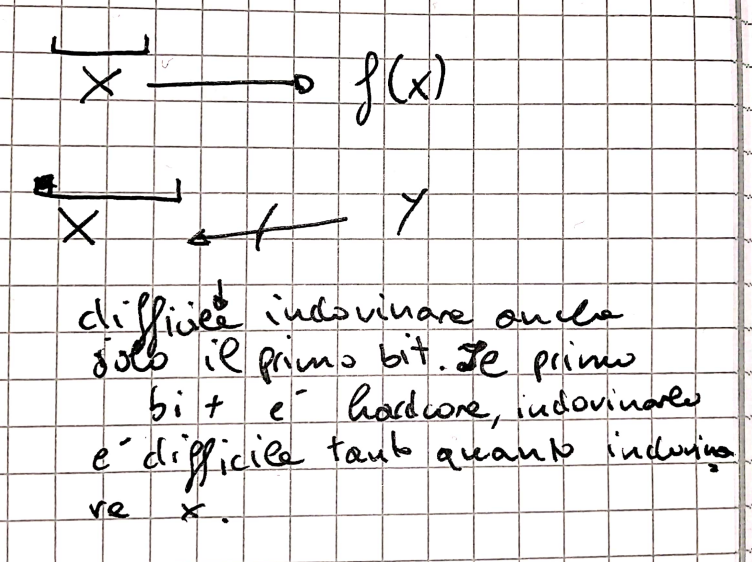
\includegraphics[width=200pt]{./img/funzioni-one-way.png}
	\caption{Quello che in breve, dobbiamo sapere su questo generatore}
	\label{img:funzioni-one-way}
\end{figure}

\newpage

\section{Generatore Blum, Blum, Shub}

\begin{figure}[htp]
	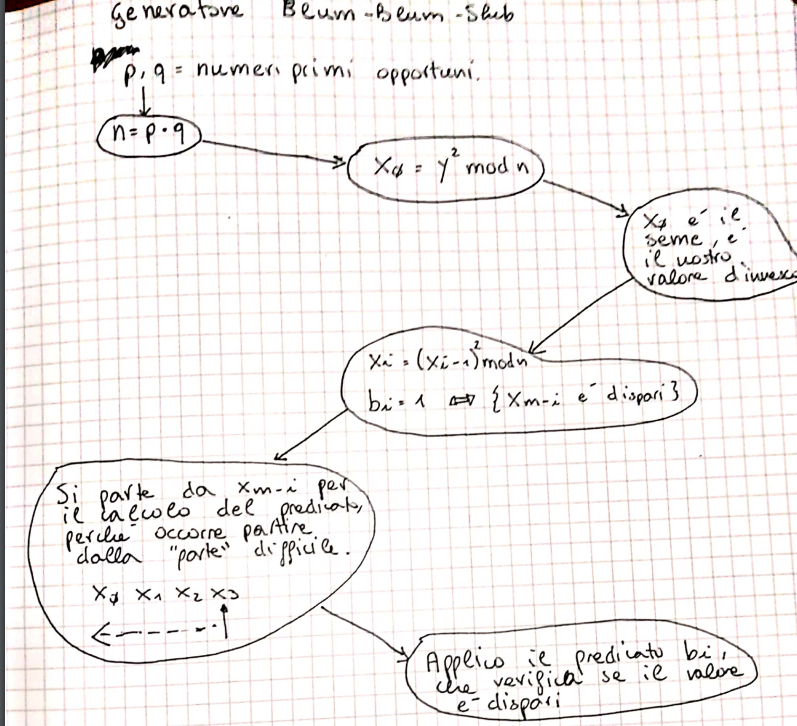
\includegraphics[width=0.8\linewidth]{./img/blumblumshub.png}
	\caption{Quello che in breve, dobbiamo sapere su questo generatore}
	\label{img:blumblumshub}
\end{figure}

	
	\chapter{DES}

\begin{lstlisting}
	//Hello.java
	import javax.swing.JApplet;
	import java.awt.Graphics;
	
	public class Hello extends JApplet {
		public void paintComponent(Graphics g) {
			g.drawString("Hello, world!", 65, 95);
		}    
	}
\end{lstlisting}
	
	\chapter{RSA}

\section{Introduzione}

Rivoluzione nel campo della crittografia, stiamo parlando di tecniche fortemente utilizzate al giorno d'oggi, ovvero di protocolli a chiave pubblica. Permette di condividere un segreto fra mittente e destinatario, nonostante non esista una chiave posso comunicare in completa segretezza. Questa rivoluzione è avvenuta negli anni 70.

\section{Descrizione}

Nei cifrari simmetrici visti sinora la chiave di cifratura è
uguale a quella di decifrazione (o comunque ciascuna può
essere facilmente calcolata dall’altra), ed è nota solo ai
due partner che la scelgono di comune accordo e la
mantengono segreta. Nei cifrari a chiave pubblica, o asimmetrici, le chiavi di cifratura e di decifrazione sono completamente diverse tra
loro. Esse sono scelte dal destinatario che rende pubblica
la chiave di cifratura k[pub], che è quindi nota a tutti, e
mantiene segreta la chiave di decifrazione k[prv] che è
quindi nota soltanto a chi la genera. Chiunque voglia spedirmi qualcosa deve conoscere la mia chiave pubblica. Esiste una coppia k[pub], k[prv] per ogni utente del
sistema, scelta da questi nella sua veste di possibile
destinatario Dest. La cifratura di un messaggio m da
inviare a Dest è eseguita da qualunque mittente come
c = C(m; k[pub]), ove sia la chiave k[pub] che la funzione
di cifratura C sono note a tutti. La decifrazione è eseguita
da Dest come m = D(c; k[prv]), ove D è la funzione di
decifrazione anch’essa nota a tutti, ma k[prv] non è
disponibile agli altri che non possono quindi ricostruire m. Il concetto base era già noto nel 76, non era invece chiara quale C e quale D avessero queste proprietà.

\section{Asimmetria}

L’appellativo di asimmetrici assegnato a questi cifrari
sottolinea i ruoli completamente diversi svolti da Mitt e
Dest, in contrapposizione ai ruoli intercambiabili che essi
hanno nei cifrari simmetrici ove condividono la stessa
informazione (cioè la chiave) segreta. 

\newpage

\section{Proprietà}

\begin{itemize}
	\item Per ogni possibile messaggio $m$ si ha:\\
	$D(C(m, k[pub]), k[prv]) = m$ \\
	Dunque stiamo dicendo che $D(C(m)) = m $, ossia Dest deve avere la possibilità di interpretare qualunque messaggio che gli altri utenti decidano di spedirgli. $C(D(m)) = m$ invece non vale sempre, chi soddisfa questa proprietà commutativa è molto apprezzato, perchè permette di implementare la firma digitale.;
	\item La sicurezza e l’efficienza del sistema dipendono dalle
	funzioni C e D, e dalla relazione che esiste tra le chiavi
	k[prv] e k[pub] di ogni coppia;
	\item La coppia k[prv] e k[pub] è facile da generare, e deve
	risultare praticamente impossibile che due utenti scelgano
	la stessa chiave deve essere inoltre praticamente impossibile (computazionalmente difficile) risalire alla chiave privata dalla pubblica.
	\item Dati m e k[pub], è facile per il mittente calcolare il
	crittogramma c = C(m, k[pub]). (deve essere facile la codifica).
	\item Dati c e k[prv], è facile per il destinatario calcolare il
	messaggio originale m = D(c, k[prv]) (deve essere facile la decodifica)
	\item Pur conoscendo il crittogramma c, la chiave pubblica
	k[pub], e le funzioni C e D, è difficile per un
	crittoanalista risalire al messaggio m, ancora peggio alla chiave privata!. Risalire al messaggio smaschera una comunicazione (violazione puntuale), risalire alla chiave privata comporta invece una violazione totale del protocollo.
\end{itemize}

\section{Sicurezza}

I protocolli a chiave privata vengono definiti sicuri in maniera empirica, ergo se non è stato violato in n anni di utilizzo è sicuro. Nei protocolli a chiave pubblica invece la sicurezza è determinata dal fatto che per violarli dovremmo riuscire a risolvere in tempo polinomiale dei problemi che fino ad esso non siamo riusciti a risolvere (non è stato possibile risolvere questo problema in anni,secoli e millenni, per questo è un certificato di garanzia di gran lunga migliore rispetto a quello dei protocolli a chiave privata).

\section{Funzioni one-way}

C deve essere una funzione one-way, cioè facile da calcolare e difficile da invertire, ma deve contenere un meccanismo segreto detto trap-door che ne consenta la facile invertibilità solo a chi conosca tale meccanismo (questo è il succo, la sintesi dei protocolli a chiave pubblica, lo svela-segreto è la chiave privata). La conoscenza di k[pub] non fornisce alcuna indicazione sul meccanismo segreto, che è svelato da k[prv] quando questa chiave è inserita nella funzione D (D = decodifica).

\section{Richiami di algebra modulare}

$\mathbb{Z}_n$ è l'insieme di numeri modulo $m$. $\mathbb{Z}^{*}_n$ è un sottoinsieme di $\mathbb{Z}_n$ e rappresenta l'insieme di elementi di $\mathbb{Z}_n$ relativamente primi con $n$, 0 ed 1 esclusi. La notazione $a$ mod $n$ significa fare a fette $a$ in chunk lunghi $n$. Se prendo due numeri e li divido per lo stesso $n$ e ottengo lo stesso resto sono nella stessa classe di equivalenza.

\begin{itemize}
	\item $\mathbb{Z}_n = \{0, 1, ..., n\}$;
	\item $\mathbb{Z}^{*}_p = \{1, ..., p - 1\}$;
	\item $a$ mod $n$ è il resto della divisione intera fra $a$ e $n$;
	\item $a$ $\cong$ $b$ mod $n$ se e solo se $a$ mod $n$ = $b$ mod $n$;
	\item $a$ $\cong$ $b$ mod $n$ se e solo se $a$ = $b + kn$; 
	\item $a$ primo con $b$ se e solo se il loro massimo comun divisore è uguale a 1.
\end{itemize}

\section{Funzione di Eulero}

Concetto importantissimo, non fa altro che dirci quanto è grande $\mathbb{Z}^{*}_n$, ovvero la sua cardinalità.Ovvero:\\\\
$\phi(n) = |\mathbb{Z}^{*}_n|$
\subsection{Proprietà}
\begin{itemize}
	\item $\phi(p) = p - 1$ 
	\item $\phi(pq) = (p - 1) (q - 1)$
	\item $a$ primo con $b$ allora $\phi(ab) = \phi(a) \phi(b)$
	\item $\phi(n)$ difficile da calcolare (non riusciamo a calcolarla efficientemente, se sapessimo fattorizzare sarebbe facile anche calcolare $\phi$. Anche se fosse difficile fattorizzare noi potremmo tentare di trovare $\phi$ con metodi alternativi).
\end{itemize}

\section{Teorema di Eulero}

Sia $n > 1$ e $a$ primo con $n$, allora:\\\\
$a^{\phi(n)} \cong 1$ mod $n$ 
	
	\chapter{DH}

\begin{lstlisting}
	//Hello.java
	import javax.swing.JApplet;
	import java.awt.Graphics;
	
	public class Hello extends JApplet {
		public void paintComponent(Graphics g) {
			g.drawString("Hello, world!", 65, 95);
		}    
	}
\end{lstlisting}
	
	\chapter{Curve ellittiche}

\begin{lstlisting}
	//Hello.java
	import javax.swing.JApplet;
	import java.awt.Graphics;
	
	public class Hello extends JApplet {
		public void paintComponent(Graphics g) {
			g.drawString("Hello, world!", 65, 95);
		}    
	}
\end{lstlisting}
	
	\chapter{Firma digitale}

\begin{lstlisting}
	//Hello.java
	import javax.swing.JApplet;
	import java.awt.Graphics;
	
	public class Hello extends JApplet {
		public void paintComponent(Graphics g) {
			g.drawString("Hello, world!", 65, 95);
		}    
	}
\end{lstlisting}
	
	\chapter{SSL}

\begin{lstlisting}
	//Hello.java
	import javax.swing.JApplet;
	import java.awt.Graphics;
	
	public class Hello extends JApplet {
		public void paintComponent(Graphics g) {
			g.drawString("Hello, world!", 65, 95);
		}    
	}
\end{lstlisting}
	
	\include{Protocolli Zero Knowledge}
	
	\chapter{Bitcoin}

\begin{lstlisting}
	//Hello.java
	import javax.swing.JApplet;
	import java.awt.Graphics;
	
	public class Hello extends JApplet {
		public void paintComponent(Graphics g) {
			g.drawString("Hello, world!", 65, 95);
		}    
	}
\end{lstlisting}
	
	\chapter{Teoria dell'informazione}

\begin{lstlisting}
	//Hello.java
	import javax.swing.JApplet;
	import java.awt.Graphics;
	
	public class Hello extends JApplet {
		public void paintComponent(Graphics g) {
			g.drawString("Hello, world!", 65, 95);
		}    
	}
\end{lstlisting}
	
	\chapter{RFID e protocolli crittografici}

\begin{lstlisting}
	//Hello.java
	import javax.swing.JApplet;
	import java.awt.Graphics;
	
	public class Hello extends JApplet {
		public void paintComponent(Graphics g) {
			g.drawString("Hello, world!", 65, 95);
		}    
	}
\end{lstlisting}
	

\end{document}